\documentclass[a4paper,10pt]{article}

%A Few Useful Packages
\usepackage{marvosym}
\usepackage{fontspec} 					%for loading fonts
\usepackage{xunicode,xltxtra,url,parskip} 	%other packages for formatting
\RequirePackage{color,graphicx}
\usepackage[usenames,dvipsnames]{xcolor}
\usepackage[big]{layaureo} 				%better formatting of the A4 page
% an alternative to Layaureo can be ** \usepackage{fullpage} **
%\usepackage{fullpage}
\usepackage{supertabular} 				%for Grades
\usepackage{titlesec}					%custom \section

%Setup hyperref package, and colours for links
\usepackage{hyperref}
\definecolor{linkcolour}{rgb}{0,0.2,0.6}
\hypersetup{colorlinks,breaklinks,urlcolor=linkcolour, linkcolor=linkcolour}

%FONTS
\defaultfontfeatures{Mapping=tex-text}
%\setmainfont[SmallCapsFont = Fontin SmallCaps]{Fontin}
%%% modified for Karol Kozioł for ShareLaTeX use
\setmainfont[
SmallCapsFont = Fontin-SmallCaps.otf,
BoldFont = Fontin-Bold.otf,
ItalicFont = Fontin-Italic.otf
]
{Fontin.otf}
%%%

%CV Sections inspired by: 
%http://stefano.italians.nl/archives/26
\titleformat{\section}{\Large\scshape\raggedright}{}{0em}{}[\titlerule]
\titlespacing{\section}{0pt}{3pt}{3pt}
%Tweak a bit the top margin
%\addtolength{\voffset}{-1.3cm}

%Italian hyphenation for the word: ''corporations''
\hyphenation{im-pre-se}

%-------------WATERMARK TEST [**not part of a CV**]---------------
\usepackage[absolute]{textpos}

\setlength{\TPHorizModule}{30mm}
\setlength{\TPVertModule}{\TPHorizModule}
\textblockorigin{2mm}{0.65\paperheight}
\setlength{\parindent}{0pt}

%--------------------BEGIN DOCUMENT----------------------
\begin{document}

%WATERMARK TEST [**not part of a CV**]---------------
%\font\wm=''Baskerville:color=787878'' at 8pt
%\font\wmweb=''Baskerville:color=FF1493'' at 8pt
%{\wm 
%	\begin{textblock}{1}(0,0)
%		\rotatebox{-90}{\parbox{500mm}{
%			Typeset by Alessandro Plasmati with \XeTeX\  \today\ for 
%			{\wmweb \href{http://www.aleplasmati.comuv.com}{aleplasmati.comuv.com}}
%		}
%	}
%	\end{textblock}
%}

\pagestyle{empty} % non-numbered pages

\font\fb=''[cmr10]'' %for use with \LaTeX command

%--------------------TITLE-------------
\par{\centering
		{\Huge Khalid \textsc{Mahmoud Mohamed Ahmed}
	}\bigskip\par}

%--------------------SECTIONS-----------------------------------
%Section: Personal Data
\section{Personal Data}
\begin{tabular}{rl}
    \textsc{Date of Birth:} & 23.07.1992   \\
		\textsc{Nationality:} & Egyptian  \\ 
    \textsc{Marital Status:} & Married  \\
    \textsc{Address:}   & Markweg 9,  \\
    & 91056 Erlangen, Germany  \\
    \textsc{Phone:}     & +4917669463160 \\
    \textsc{email:}     & engkhalid.mahmoud92@gmail.com \\
    &
\end{tabular}
\begin{textblock}{2.5}(4.5,-4.75)
	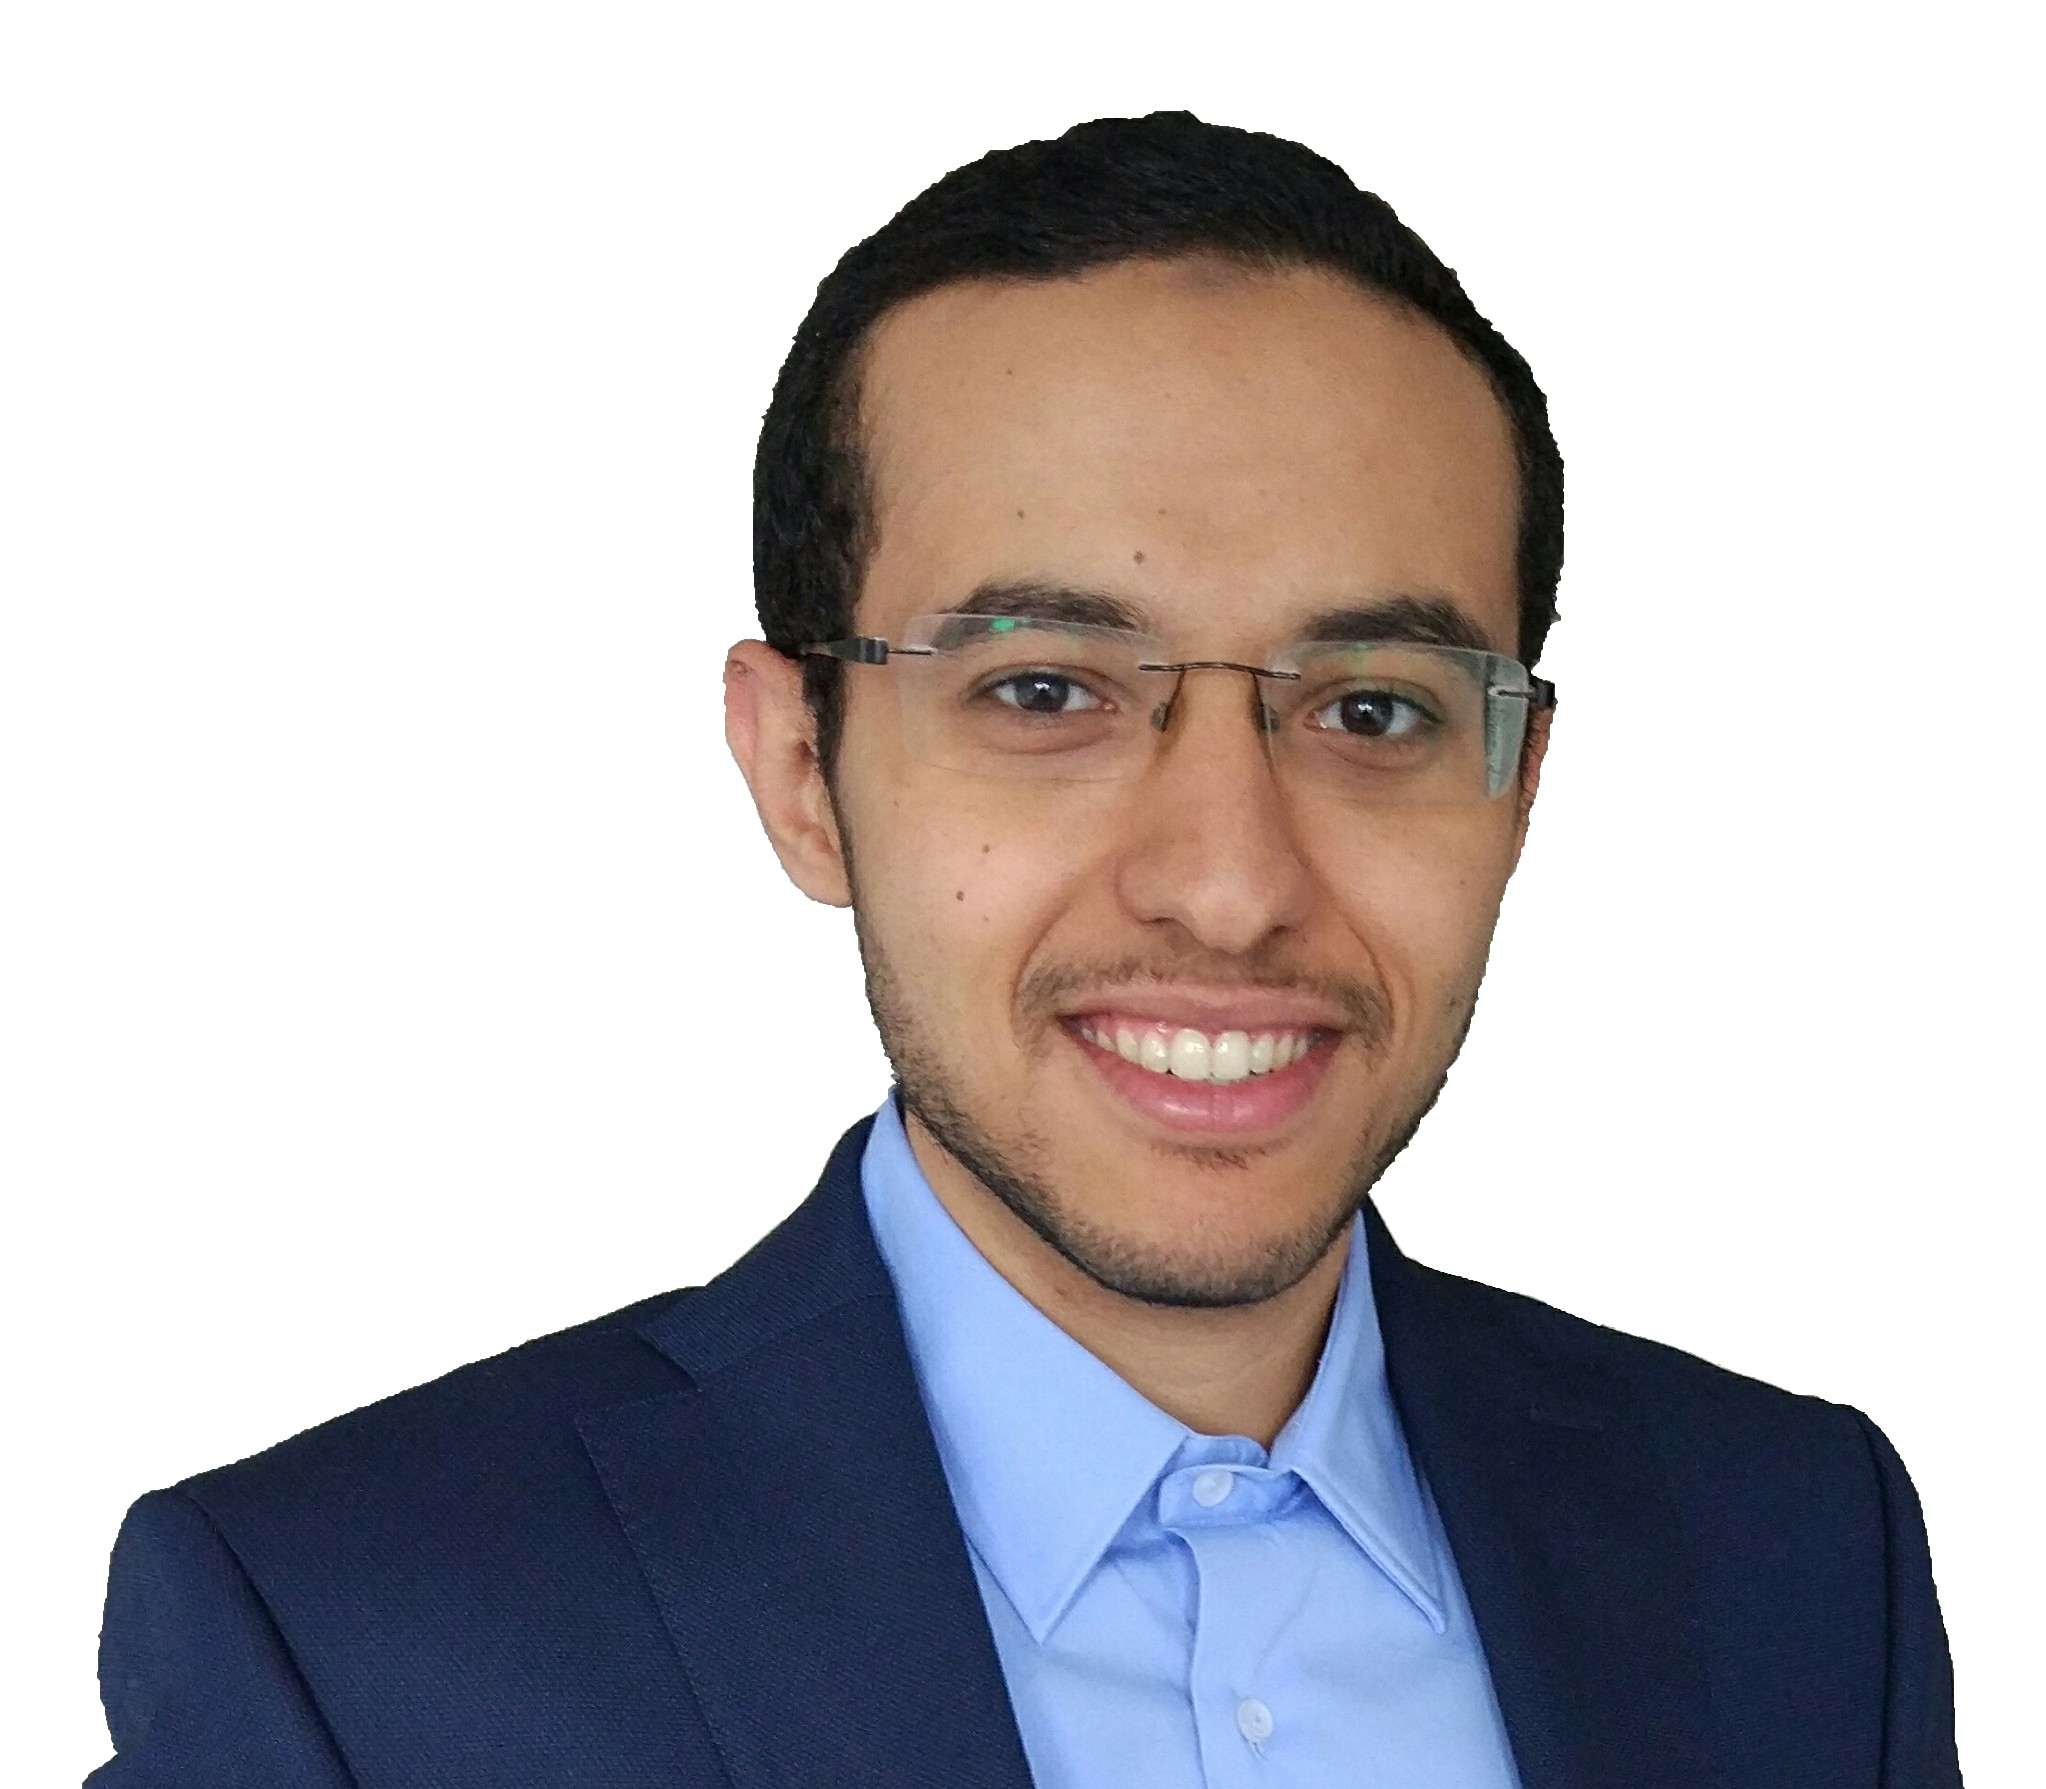
\includegraphics[width=4.5cm,height=4.2cm]{khalid.jpg}
\end{textblock}
%Section: Education
\section{Education}
\begin{tabular}{r|p{9cm}}	
\textsc{Oct.} 2014 - \textsc{June} 2017 & Masters of Science student in Communication and Multimedia Engineering at the {\bf Friedrich-Alexander-University}, Erlangen, Germany (GPA 1.6/1.0). \\
& \\

 \textsc{July} 2014 & Bachelor of Science in Information Engineering and Technology with High Honors at the {\bf German University in Cairo}, Egypt (GPA 1.08/0.7)\\
& \\
 \textsc{Sept.} 2007 - \textsc{July} 2009 & {\bf Dr.Mahmoud Omar Secondary School}, Egypt
\end{tabular}

\section{Work Experience}
\begin{tabular}{r|p{9cm}}
	\textsc{June} 2017 - still running & Research engineer at {\bf Fraunhofer für Integrierte Schaltungen IIS}.\\
	& Implementing short transmission time interval (sTTI) physical layer features for LTE release 15 on openairinterface (OAI) -open source- platform. \\
	& Implementing a New Radio/5G (NR) uplink system level simulator with a focus on Ultra Reliable Low Latency Communication (URLLC) use case. The implementation is done using MATLAB object oriented programming.\\	
	\textsc{January} 2015 - \textsc{April} 2016 & Student research assistant (Hiwi) in RFID Project at LIKE, {\bf Friedrich-Alexander-University}.\\
	& Implementing a maximum likelihood (ML) receiver for RFID tag reader using multiple receive antennas using MATLAB. \\
	& Validating the performance of ML receiver in a multiple input-multiple output (MIMO) double rayleigh backscatter channel. \\ 
\end{tabular}

\section{Internships}
\begin{tabular}{r|p{11cm}}
	\textsc{May 2016 – Oct. 2016} & Internship at {\bf Fraunhofer IIS}. The task was to develop and enhance the {OAI} simulation environment to allow for shorter transmission time intervals ({TTI}) in LTE release 15 on the physical layer in the downlink using {\bf C} programming language. The task was a step towards development of 5G NR. A 7-OFDM symbol downlink {sTTI} was developed and tested using OAI simulation environment. \\
	& \\ 
	\textsc{Oct. 2012 – Jan. 2013} & Junior teaching assistant at the {\bf German university in Cairo} teaching CSIS104 for pharmacy students and CSEN102 for engineering students. \\
	& \\
	\textsc{August} 2012 & "Wireless communication" internship at the {\bf German University in Cairo} learning to work on tinyos to program mib510 motes using \textbf{nesC} programing language on ubuntu then implementing a simple application about indoor localization using Finger Printing algorithm.\\
	& \\
	\textsc{July} 2012 & "Radio Frequency" (RF) internship at the {\bf German University in Cairo}, designing and simulating RF couplers ,filters and phase shifter using  Computer Simulation Technology (CST).\\ 
	& \\
	\textsc{July} 2011 & Summer Internship at the {\bf Biomedical Inistitute, Technical University in Ilmenua}, Germany, designing a flash-light control system by programming Texas micro controller using \textbf{C} language.\\ 
	& \\
	\textsc{July} 2010  & Summer Internship at the {\bf Biomedical Inistitute, Technical University in Ilmenua}, Germany, designing and fabricating simple printed circuit boards (PCBs).\\
	
\end{tabular}

%Section: Research
\section{Research}
\begin{tabular}{r|p{9cm}}
\textsc{March} 2018 - \textsc{Sept.} 2018 & ٍٍSupervision of a bachelor thesis student at {\bf Fraunhofer-Institut IIS}. "Uplink grant free transmission for reliable communications", New features were added to the system level simulator which was implemented during my master thesis, to evaluate collision probability and blind detection in NR grant free scheme.\\
\textsc{Oct.} 2016 - \textsc{May} 2017 & Master Thesis at the {\bf Friedrich-Alexander-University}, Erlangen, Germany in collaboration with {\bf Fraunhofer-Institut für Integrierte Schaltungen IIS}. "Uplink Multiple Access Schemes for Ultra-Low Latency Transmission", A system-level simulator is implemented using MATLAB object oriented programming simulation environment to test different proposals to guarantee fast access and high reliability to low latency users in LTE.\\
 \textsc{March} 2013 - \textsc{Sept.} 2013 & Bachelor Project at the {\bf Technical University in Ilmenau}, Germany. "Wireless Health Monitoring System Based on Fiber-Optic Sensors", a wireless portable system to measure the respiratory rate using a fiber Bragg grating (FBG) optical sensor is established. Analyzing and filtering the output data is explained and compared with the output data of a commercial piezoelectric sensor.\\
\end{tabular}
%Section: Work Experience at the top






%Section: Languages
\section{Languages}
\begin{tabular}{rl}
\textsc{Arabic:}&Mother Tongue\\
\textsc{English:}&Fluent\\
\textsc{German:}&B1.2\\
\end{tabular}

\section{Computer Skills}
\begin{tabular}{rl}
Very Good Knowledge:& \textsc{MATLAB} \\
Intermediate Knowledge:& C and Version Control Systems: git \\
Basic Knowledge:& Linux, \textsc{java}, \textsc{CST - Computer Simulation Technology} and Mathematica
\end{tabular}

\section{Interests and Activities}
\subsection*{Interests}
Wireless communications , cellular networks and software development.\\
\subsection*{Activities}
Football, Tennis and Cycling


%\newpage
%\hypertarget{gmat}{\textsc{Gmat}\setmainfont{LMRoman10 Regular}\textregistered\setmainfont[SmallCapsFont=Fontin-SmallCaps]{Fontin-Regular}}

%\XeTeXpdffile ''GMAT.pdf'' page 1 scaled 800

\end{document}
